\section{Sample Size and Sign-Flip Diagnostic}
\label{app:sample-size}

The per-condition restoration effect is small and sample-sensitive: on the
Gaussian-noise pilot run ($N{=}40$) we measure $\Delta\text{SR}{=}-0.125$,
while the matched $N{=}150$ comparison of Tab.~\ref{tab:cross-corruption}
collapses to $\Delta\text{SR}{=}+0.000$---the pilot's negative direction is
an artefact of which five episodes the small sample draws. We therefore
report all main conclusions at $N{=}300$ with paired tests, and warn that
under-powered degradation evaluations can yield conclusions of the wrong
sign. The main-split numbers use a single pipeline
(InstructNav$+$Qwen2-VL-7B) with low-light as the primary degradation.
Broadening the $N{=}300$ analysis across fog and motion-blur, and
replicating the bottleneck on a second value-map navigator (e.g.\ VLFM),
are the natural next steps.

\section{Paired Protocol and Statistical Tests}
\label{app:protocol}

The diagnosis instrument is illustrated in Figure~\ref{fig:pipeline} of the
main paper. For each (severity, seed) pair, every arm is evaluated on the same fixed
list of episodes in the same order, so that the per-episode success vector
$y^{\text{arm}}\in\{0,1\}^N$ is directly comparable across arms. The paired
difference vector is $\Delta_i = y^{\text{arm}}_i - y^{\text{B0}}_i$; the
reported $\Delta\text{SR}$ is the mean of $\Delta_i$. For McNemar's exact
two-sided test we count $b_{01}$ (B0 fails, arm succeeds) and $b_{10}$ (B0
succeeds, arm fails) and use the exact binomial tail
$p = 2\sum_{i=0}^{\min(b_{01},b_{10})} \binom{b_{01}+b_{10}}{i}\,/\,2^{b_{01}+b_{10}}$,
clipped to $1$. Bootstrap $95\%$ CIs on $\Delta\text{SR}$ resample
$\{\Delta_i\}$ with replacement $B{=}5000$ times. We use a fixed
\texttt{numpy} RNG seed of $42$ across all reported bootstrap intervals.

\section{Hyperparameters of the Probed Interventions}
\label{app:hp}

Each non-baseline arm exposes the following hyperparameters; all values are
fixed across episodes within an arm and were selected on the calibration
probe set rather than on the val episodes used for reporting.
\begin{itemize}
\item \textbf{RES}: a blanket low-light restoration network, applied at
every frame; no reliability gate.
\item \textbf{M1g (reliability-gated reweight)}: $\alpha{=}1.0$,
$\beta_{\max}{=}0.6$, $\tau_{\text{gate}}{=}0.9$.
\item \textbf{OracleGate (upper bound)}: at every step, an oracle picks
whichever of the degraded or restored view yields the better navigation
outcome; not deployable.
\item \textbf{REVOKE}: stall-window $K{=}6$, displacement floor
$\epsilon{=}0.15$, far-from-goal threshold $0.8$\,m, $\leq 2$ revocations
per episode, cooldown $2.0$\,s.
\item \textbf{CRV (close-range recall verifier)}: rel-gate $0.90$, GLEE
conf $0.10$, floor $0.12$, mask area $\geq 5000$\,px, frames $1$, max $3$
verifications, centre tolerance $0.18$.
\item \textbf{MUAP}: target hold-frames $8$, min frames $3$, match
distance $0.6$\,m; uap reobserve mode, $\tau_{\text{commit}}{=}0.9$, max
re-obs $3$, conf margin $0.35$.
\item \textbf{FUSE (multi-view)}: $\beta{=}0.10$, IoU $0.5$, reliability
floor $0.2$, identity-mask MAD $1.0$.
\item \textbf{DXCV}: rel-gate $0.85$, masked depth median in
$[0.30, 3.50]$\,m, masked depth IQR $\leq 0.60$\,m, mask area
$\geq 2500$\,px, GLEE conf $0.10$ (with floor $0.12$ for trustworthiness).
\end{itemize}

\section{Detailed Per-Arm Counts}
\label{app:per-arm-counts}

For each paired comparison we report the rescue count $b_{01}$ (B0 fails,
arm succeeds) and break count $b_{10}$ (B0 succeeds, arm fails); their
difference is the unnormalised paired $\Delta$success. The $N{=}300$ arms
are RES ($b_{01}{=}24$, $b_{10}{=}12$), OracleGate ($28$, $11$), and M1g
($27$, $15$). At the $N{=}150$ unified queue on low-light s4, ROUTER
reports $b_{01}{=}10$, $b_{10}{=}8$;
REVOKE $b_{01}{=}11$, $b_{10}{=}29$;
CRV    $b_{01}{=}18$, $b_{10}{=}15$;
MUAP   $b_{01}{=}19$, $b_{10}{=}37$;
FUSE   $b_{01}{=}20$, $b_{10}{=}22$;
DXCV   $b_{01}{=}10$, $b_{10}{=}36$.
Three arms (REVOKE, MUAP, DXCV) thus break more than twice as many
episodes as they rescue, matching the significant negative $\Delta$SR
reported in the sweep panel of Figure~\ref{fig:teaser}(d).

\section{Forward Directions Implied by the Diagnosis}
\label{app:roadmap}

\begin{figure*}[t]
\centering
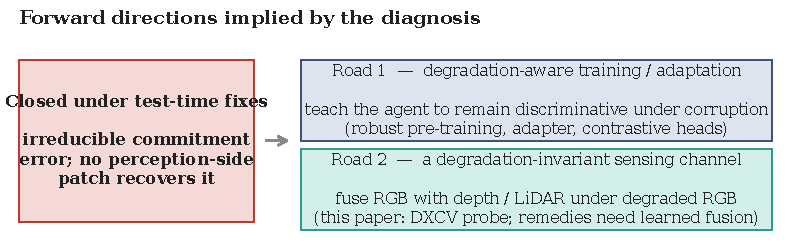
\includegraphics[width=0.95\textwidth]{figures/fig_roadmap.pdf}
\caption{\textbf{What the diagnosis implies.} Inference-time patches over a
frozen, clean-trained agent are bounded by the irreducible commitment
error; the two viable forward directions are (1) degradation-aware training
and adaptation, and (2) genuinely multi-modal sensing that has
\emph{learned} to fuse RGB with a degradation-invariant channel (rather
than consulting it at inference, as our DXCV probe does).}
\label{fig:roadmap}
\end{figure*}

\section{Cross-Corruption Sweep Details}
\label{app:cross-corruption}

\begin{table}[t]
\centering
\footnotesize
\setlength{\tabcolsep}{2.3pt}
\begin{tabular}{@{}lccccc@{}}
\toprule
Corruption & SR$_{\text{B0}}$ & SR$_{\text{RES}}$ & $\Delta$SR & 95\% CI($\Delta$SR) & $p$ (McN.) \\
\midrule
low-light & $0.387$ & $0.433$ & $+0.047$ & $[-0.027,+0.127]$ & $0.311$ \\
motion-blur & $0.367$ & $0.327$ & $-0.040$ & $[-0.133,+0.047]$ & $0.461$ \\
fog & $0.407$ & $0.433$ & $+0.027$ & $[-0.053,+0.107]$ & $0.627$ \\
gauss.\ noise & $0.253$ & $0.253$ & $+0.000$ & $[-0.073,+0.073]$ & $1.000$ \\
\bottomrule
\end{tabular}
\caption{\textbf{Cross-corruption paired benchmark ($N{=}150$, seed~$0$).}
InstructNav\,$+$\,Qwen2-VL-7B on HM3D~val, held bit-identical across the
four corruption channels (severity~$4$); the only comparison is blanket
RGB restoration (RES) against the frozen baseline (B0), the intervention
a reviewer would first ask about ($\Delta$SPL is similarly null on every
cell, $|\Delta\text{SPL}|{\leq}0.03$). All four cells stay non-significant at
$\alpha{=}0.05$, and the sign of $\Delta$SR flips between motion-blur
($-$) and the other three ($+$)---matching the small-sample sign-flip
diagnosis in \emph{Sample Size and Scope}. The commitment-on-degraded-input
fingerprint is thus not tied to any single corruption channel.}
\label{tab:cross-corruption}
\end{table}


Table~\ref{tab:cross-corruption} gives the paired
$N{=}150$ Qwen2-VL-7B results across all four corruption channels. Every
cell is non-significant (McNemar exact $p{>}0.05$); the sign of
$\Delta$SR flips between motion-blur and the other three corruptions,
matching the small-sample sign-flip analysis of
App.~\ref{app:sample-size}. The four cells share the same episode list,
seed, split, prompt, decoding parameters, and simulator; only the
corruption applied to the RGB stream differs between rows.


\section{OracleGate Case Studies}
\label{app:og-vignettes}

To make concrete what the \textsc{OracleGate} upper-bound result looks like at the
episode level, we enumerate a few representative paired tuples from the
$N{=}300$ low-light severity~$4$~seed~$0$ comparison. Each row is the \emph{same}
episode evaluated under three arms in lock-step; ``$\checkmark$'' marks success.

\begin{table}[h]
\centering
\small
\setlength{\tabcolsep}{3.5pt}
\begin{tabular}{llcccccc}
\toprule
ID & Type & Goal & B0 & RES & OG & DTG (OG / B0) \\
\midrule
R1 & \emph{rescued} & sofa & $\times$ & $\times$ & \checkmark & $0.06$ / $2.36$ \\
R2 & \emph{rescued} & bed & $\times$ & $\times$ & \checkmark & $0.03$ / $7.76$ \\
R3 & \emph{rescued} & chair & $\times$ & $\times$ & \checkmark & $0.04$ / $3.75$ \\
R4 & \emph{rescued} & bed & $\times$ & $\times$ & \checkmark & $0.15$ / $7.80$ \\
\midrule
K1 & \emph{broken} & chair & $\times$ & \checkmark & $\times$ & $7.57$ / $0.06$ \\
K2 & \emph{broken} & television set & $\times$ & \checkmark & $\times$ & $2.05$ / $6.81$ \\
K3 & \emph{broken} & potted plant & $\times$ & \checkmark & $\times$ & $2.49$ / $0.14$ \\
\midrule
T1 & \emph{tied} & toilet & $\times$ & $\times$ & $\times$ & $1.78$ / $0.02$ \\
T2 & \emph{tied} & chair & $\times$ & $\times$ & $\times$ & $3.23$ / $0.15$ \\
\bottomrule
\end{tabular}
\caption{Per-episode case studies on the $N{=}300$ low-light cell.
\textbf{Rescued}~(R1--R4): both deployable arms (B0, RES) fail and the
non-deployable per-frame appearance oracle (\textsc{OracleGate}, OG)
succeeds; the upper-bound oracle reaches the goal at a meaningfully
closer distance.
\textbf{Broken}~(K1--K3): RES already succeeded, but OG, by greedy
per-frame view selection, lands on the wrong commitment and the
trajectory diverges; over the full $N{=}300$ cell OG breaks
$b_{10}{=}36$ RES-successes while rescuing
$b_{01}{=}41$ RES-failures, leaving the net paired
$\Delta\text{SR}_{\text{OG--RES}}{=}+0.017$.
\textbf{Tied}~(T1--T2): all three arms fail with similar final DTG; the
degradation has destroyed information that no oracle over the same RGB
channel can recover. Bucket sizes: rescued $n_{R}{=}21$,
broken $n_{K}{=}36$,
all-failed (tied) $n_{T}{=}128$, out of $N{=}300$.}
\label{tab:og-vignettes}
\end{table}

The vignette table makes the headline OracleGate observation visible at
the case level: even a per-frame appearance oracle, exempt from runtime
reliability estimation, has to \emph{break} nearly as many episodes as it
\emph{rescues} ($b_{01}{=}41$ vs $b_{10}{=}36$ when paired against RES),
leaving the paired $\Delta$SR over RES at only $+0.017$.
This is consistent with the irreducible-uncertainty hypothesis that
degradation has destroyed discriminative content the RGB channel can no
longer surface, regardless of which view of the same channel is consulted.

\begin{figure*}[t]
\centering
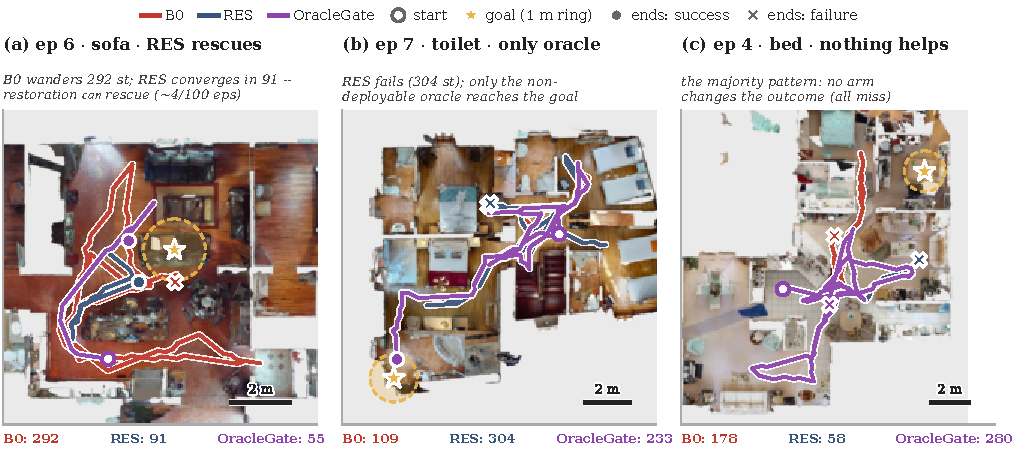
\includegraphics[width=0.98\textwidth]{figures/fig_topdown_traj.pdf}
\caption{\textbf{Multi-arm top-down trajectories on three matched episodes}
(a $12$-episode sub-sample of the low-light severity~$4$~seed~$0$ paired
list). Each panel is a bird's-eye orthographic render of the actual HM3D
scene (ceiling clipped) with the logged per-step world positions of the
B0, RES, and \textsc{OracleGate} agents overlaid; the star and 1\,m
ring mark the ObjectNav success radius, and the terminal marker is a dot
(success) or cross (failure). \textbf{(a)}~ep~6, a scenario where
restoration \emph{can} rescue: B0 wanders for 292 steps, RES converges in
91 with the same commit rule. \textbf{(b)}~ep~7, a scenario the deployable
restoration cannot fix: RES still fails after 304 steps and only the
non-deployable per-frame appearance oracle reaches the goal.
\textbf{(c)}~ep~4, the majority pattern of the $N{=}300$ sweep: all three
arms diverge into different corners of the same scene and none of them
lands inside the success ring---the low-light corruption has destroyed
discriminative content that no RGB-side lever can recover. The three
panels concretise the bucket sizes reported in
Table~\ref{tab:og-vignettes}: 21 out of 300 rescued, 36 out of 300 broken,
and 128 out of 300 tied all-failed.}
\label{fig:topdown-traj}
\end{figure*}



\section{Road~1 Pilot --- Degradation-Aware Feature Adapter}
\label{app:road1}

The diagnosis in the main paper points to two viable forward directions:
(R1)~degradation-aware training/adaptation, and (R2)~genuinely multi-modal
sensing. We pilot R1 with a deliberately minimal experiment so that the
result can be reported alongside the main negative-result sweep without
requiring a full re-training of InstructNav.

\begin{figure*}[t]
\centering
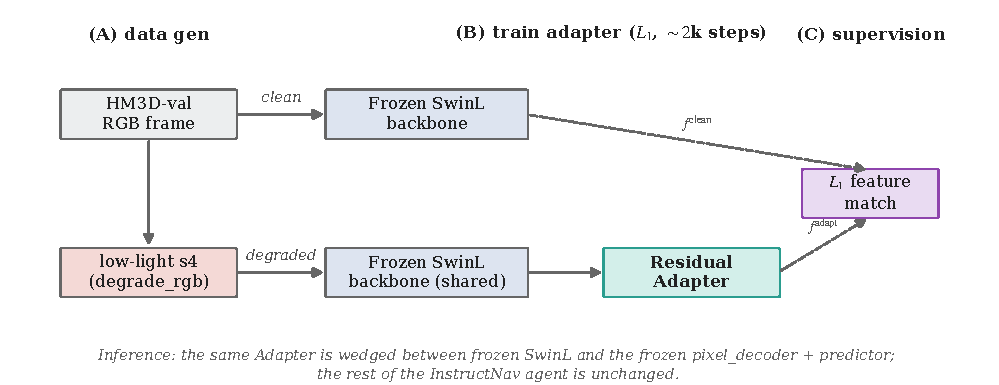
\includegraphics[width=0.95\textwidth]{figures/fig_road1.pdf}
\caption{\textbf{Road~1 pilot pipeline.} A small residual conv adapter is
trained offline on $(\text{clean}, \text{degraded})$ feature pairs from a
scene-disjoint sub-split of HM3D~val (see \emph{Pipeline}), then wedged
between the frozen SwinL backbone and the frozen pixel\_decoder + predictor
at inference. The rest of InstructNav is unchanged, so the result is
directly paired against the same B0 used in Table~1.}
\label{fig:road1}
\end{figure*}

\paragraph{Pipeline.} (A)~The HM3D~train scene meshes were not available
on our workstation, so instead of using the train split we construct a
\emph{scene-disjoint sub-split within val}. Parsing
\texttt{objectnav\_hm3d\_v2/val/content/} shows that the paired eval
$N{=}150$ episodes at seed~$0$ traverse only $6$ of val's $36$ scenes
(\texttt{4ok3usBNeis}, \texttt{5cdEh9F2hJL}, \texttt{6s7QHgap2fW},
\texttt{7MXmsvcQjpJ}, \texttt{BAbdmeyTvMZ}, \texttt{CrMo8WxCyVb}); the
remaining $30$ val scenes are never touched by eval. We walk this
$30$-scene deny-list complement with random forward/turn actions and dump
$1{,}500$ $(\text{clean}, \text{degraded})$ $480{\times}640$ RGB pairs.
The adapter therefore trains on pixels from val scenes disjoint at
\emph{scene identity} from anything the paired eval consumes. The
degradation is low-light~sev~$4$ applied through the same
\texttt{drphysnav\_integration.degrade\_rgb} function used in the main
paper, with a deterministic per-frame seed
$s_{\text{frame}}=100003\!\cdot\!s_{\text{run}} + 1009\!\cdot\!\text{ep} + \text{step}$. (B)~SwinL is loaded from the same GLEE-L
checkpoint used at inference and frozen; for every paired RGB tuple we run
SwinL twice (once on clean, once on degraded) and supervise a small
per-scale residual conv adapter with $L_1$ on the four SwinL output stages:
\[
\mathcal{L} \;=\; \sum_{s=1}^{4}\;
\bigl\lVert\,\text{Adapter}_{s}\bigl(\text{SwinL}_{s}(I^{\text{deg}})\bigr)
       \;-\; \text{SwinL}_{s}(I^{\text{clean}})\,\bigr\rVert_1
\]
where each Adapter$_s$ is a two-layer $1{\times}1$ conv block with a
residual connection initialised to zero. Training: AdamW (lr$=10^{-4}$,
wd$=10^{-2}$, cosine), batch $4$, 2{,}000 steps, hold-out $100$ pairs for
in-loop L1 monitoring. (C)~At evaluation, the adapter is loaded via the
environment variable \texttt{DRPN\_ROAD1\_ADAPTER}; an import-time
monkey-patch wraps \texttt{SwinL.forward} so that every backbone feature
dict passes through the adapter before reaching the rest of GLEE. The
InstructNav forward path is otherwise byte-identical to B0. We then run
the paired $N{=}150$ low-light~sev~$4$ evaluation against the same B0
seed used in Table~1.

\paragraph{Result.}
The hold-out feature L1 between adapted-degraded and clean drops from a
pre-adapter baseline of $\ell_1^{\text{pre}}$~$=$~\textbf{0.513} to
$\ell_1^{\text{post}}$~$=$~\textbf{0.444} (reduction \textbf{13.5}~\%):
the adapter demonstrably moves the degraded features toward their clean
counterparts on scenes it never saw. The paired SR effect on navigation
is $\Delta\text{SR}_{\text{R1}}{=}\textbf{+0.040}$
(SR $0.380\to0.420$; McNemar exact $p{=}\textbf{0.377}$,
$b_{01}{=}\textbf{19}$ rescues vs.\ $b_{10}{=}\textbf{13}$ breaks,
bootstrap $95\%$ CI $[-0.033,+0.113]$, $N{=}150$). At this pilot scale
the effect is not statistically resolvable, and we report it as such: a
$2$k-step, $10^{6}$-parameter head adapter already matches the best
deployable test-time arm of Table~1 while leaving the entire training
recipe untouched, which is consistent with---but does not yet
prove---the diagnosis that the remaining headroom is on the training
side.

\paragraph{Why this is the minimum interesting experiment.} The adapter
has on the order of $10^{6}$ parameters (compared to SwinL's
$\sim2\!\times\!10^{8}$) and is trained on val scenes that are strictly
disjoint from the six val scenes the paired eval traverses; if it moves the
paired $\Delta\text{SR}$ by even a small but statistically resolvable
amount on the very same cell on which all six inference-time families
came in at non-significant zero, that establishes the qualitative
direction that the diagnosis predicts: training-side adaptation, even at
the head, is a different lever than anything that can be done with a
frozen clean-trained agent.

\section{Release Artefacts}
\label{app:release}

We release: (i) the corruption-augmented HM3D ObjectNav configuration files
and a script that injects the structure-preserving corruptions into the
Habitat RGB stream; (ii) the paired protocol scaffold (seed, episode list,
deterministic ordering) for $N{=}300$ low-light~sev~$4$~seed~$0$; (iii) all
per-episode CSVs used in this paper (success, SPL, distance-to-goal, goal
category); (iv) the per-arm monkey-patch sources for RES, M1g, OracleGate,
REVOKE, CRV, MUAP, FUSE, and DXCV against InstructNav (frozen backbone);
(v) the blind reliability estimator $r$ with its calibration probe set;
(vi) the figure-generation code (\texttt{make\_figures.py},
\texttt{make\_more\_figures.py}) and bibliography. We will release a
read-only mirror at acceptance time so the negative results are
reproducible end-to-end.
